\documentclass[11pt]{article}
\usepackage[review]{acl}
\usepackage{times}
\usepackage{latexsym}
\usepackage[T1]{fontenc}
\usepackage[utf8]{inputenc}
\usepackage{microtype}
\usepackage{graphicx}
\usepackage{booktabs}
\usepackage{amsmath}
\usepackage{amssymb}
\usepackage{multirow}
\usepackage{xcolor}
\usepackage{subcaption}
\usepackage{enumitem}

\newcommand{\irtfit}{\textsc{IRT-FIT}}

\graphicspath{{../figures/paper/}}

\title{What Can IRT Person-Fit Statistics Reveal About SFT-Stage Benchmark Contamination?}

\author{Anonymous}

\begin{document}
\maketitle

\begin{abstract}
Benchmark contamination in Large Language Models (LLMs) undermines evaluation validity, yet most detection methods require privileged access to training data, model internals, or output probabilities.
We present the first controlled characterization of Item Response Theory (IRT) person-fit statistics for detecting supervised fine-tuning (SFT) contamination, requiring only binary response patterns and calibrated four-parameter logistic item parameters; diagnostic $\theta$-anchoring requires a clean baseline.
A contaminated LLM produces aberrant response patterns analogous to a test-taker with item preknowledge.
Using $\ell_z^*$ in a matched-difference design ($\Delta\ell_z^*$) across three 7--8B model families ($n{=}10$ clean seeds per family) on MMLU (14,042 items) and ARC-Challenge (295 items), we identify three boundaries:
(1) model-specific $\theta$-shift dynamics, where contamination-induced ability inflation absorbs the person-fit signal; $\theta$-anchoring amplifies detection by 2.4$\times$ while reducing coefficient of variation from 60\% to 19\%;
(2) a detection-diagnosis tradeoff where simpler statistics yield stronger detection but lack $\ell_z^*$'s diagnostic capabilities (seen/unseen decomposition, mechanistic $\theta$-shift analysis);
and (3, exploratory) ability-dependent non-monotonic dose-response under free-$\theta$ estimation, driven by $\theta$-shift absorption; $\theta$-anchored analysis reveals stable positive dose-response.
These findings establish when and why binary response patterns carry contamination information beyond aggregate accuracy.

\end{abstract}

\section{Introduction}\label{sec:introduction}

\begin{figure*}[t]
  \centering
  
\includegraphics[width=\textwidth]{fig_1_composite.pdf}
  \caption{Overview of IRT person-fit detection. (a)~A clean model's responses track the IRT-predicted probability curve; (b)~a contaminated model shows anomalous successes on hard items (red diamonds), producing a large $|\Delta\ell_z^*|$. (c)~Effect-size landscape: baseline accuracy vs.\ Cohen's $|d|$ across model families (diamonds: 5\%, triangles: 15\%, squares: 25\%, circles: 50\%; multi-seed means where available, single-seed otherwise; values from Table~\ref{tab:cohens_d}). (d)~Dose-response trajectories; free-$\theta$ shows non-monotonic artifact, fixed-$\theta$ recovers consistent positive dose-response.}
  \label{fig:composite}
\end{figure*}

\begin{figure*}[t]
  \centering
  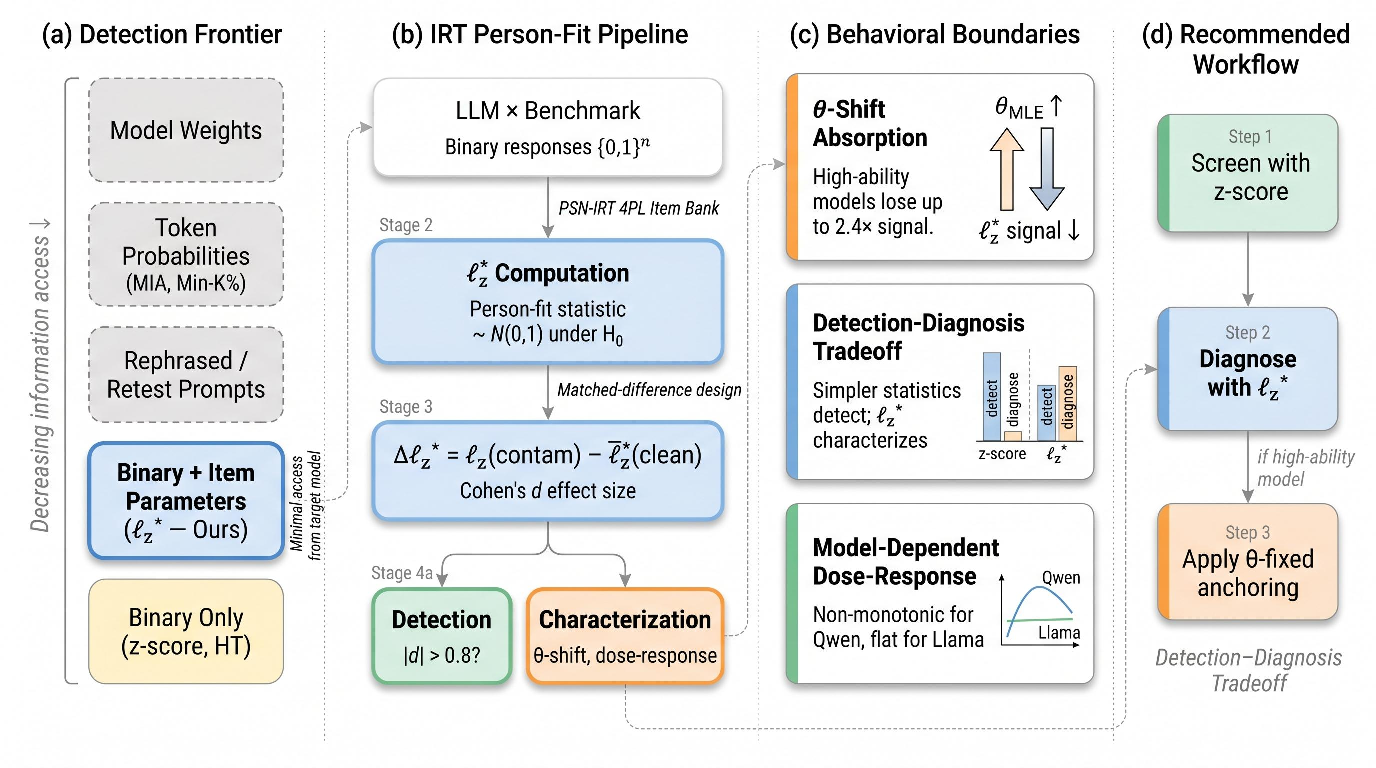
\includegraphics[width=\textwidth]{fig_framework.pdf}
  \caption{Overview of \irtfit{}: (a)~positioning in the detection frontier by information access; (b)~pipeline from binary responses through $\ell_z^*$ person-fit analysis to detection and characterization; (c)~three behavioral boundaries discovered; (d)~recommended practitioner workflow.}
  \label{fig:pipeline}
\end{figure*}

Benchmark contamination (the unintended inclusion of evaluation data in training corpora) poses a growing threat to LLM evaluation integrity \citep{dodge2021, magar2022, sainz2023}, as the probability of overlap increases structurally with expanding corpora and benchmarks \citep{jacovi2023, chang2024survey}.
Existing detection methods all require privileged access beyond binary response records: training corpora, token-level probabilities, crafted prompts, or multiple test variants (\S\ref{sec:related_work}).
Moreover, all log-probability-based detectors fail after RL post-training \citep{wang2025fragility}, motivating the question: \emph{what can binary response patterns alone reveal about contamination?}

A contaminated LLM is functionally analogous to a test-taker with item preknowledge: both produce response patterns where difficult items are answered correctly through memorization rather than genuine ability (Figure~\ref{fig:composite}a--b).
This connection points to person-fit statistics from psychometric cheating detection \citep{drasgow1985, snijders2001, karabatsos2003}.
We focus on SFT-stage contamination, where benchmark answers are explicitly included in fine-tuning data, as it provides controlled ground truth and is increasingly relevant as fine-tuning-as-a-service platforms proliferate (Figure~\ref{fig:pipeline}).

Using $\ell_z^*$ in a matched-difference design across three 7--8B model families (Qwen2.5-7B, Llama-3.1-8B, Mistral-7B; $n{=}10$ clean seeds each) with pre-calibrated four-parameter logistic (4PL) item parameters \citep{psnirt2026} on MMLU \citep{hendrycks2021mmlu} and ARC-Challenge, we identify three behavioral boundaries:

\begin{enumerate}[leftmargin=*,nosep]
\item \textbf{Model-specific $\theta$-shift dynamics.} Contamination inflates ability estimates ($\hat{\theta}$), absorbing the person-fit signal; $\theta$-anchoring amplifies Qwen's multi-seed $|d|$ by 2.4$\times$ at 50\% contamination while reducing inter-seed coefficient of variation (CV) from 60\% to 19\%, establishing $\theta$-anchoring as a necessary condition for reliable detection of high-ability models at high contamination. ARC-C reverses through a ceiling effect.

\item \textbf{Detection-diagnosis tradeoff.} Simpler statistics yield stronger detection: accuracy $z$-scores produce $|d|$ values several-fold to over an order of magnitude larger than person-fit statistics, and the nonparametric HT statistic \citep{vanderflier1982} generally exceeds $\ell_z^*$. Yet the diagnostic power reverses: only $\ell_z^*$ supports seen/unseen decomposition, mechanistic $\theta$-shift analysis, and sensitivity to response-pattern structure (57/60 vs.\ 4/60 flagged cells on real-world data).

\item \textbf{Non-monotonic dose-response under free-$\theta$ (exploratory).} The Qwen dose-response ($|d|$: $4.15 \to 5.36 \to 7.44 \to 5.08$ at 5\%/15\%/25\%/50\%; 5\% is single-seed, remainder are multi-seed means) shows non-monotonicity; $\theta$-anchoring eliminates the pattern and reveals a broadly increasing dose-response ($|d|{=}12.32$ at 50\%). The non-monotonicity is a $\theta$-estimation artifact, not a detection boundary.
\end{enumerate}

Our contributions are threefold:
(1) We provide the first empirical characterization of IRT person-fit behavior for LLM contamination, quantifying theoretically predicted phenomena ($\theta$-shift absorption, detection-diagnosis tradeoff) whose magnitudes and boundary conditions are not derivable from IRT theory alone.
(2) We establish that $\Delta\ell_z^*$ reliably detects SFT-stage contamination across three model families (all single-seed bootstrap 95\% CIs exclude zero, $n{=}10$).
(3) We document the detection-diagnosis tradeoff, clarifying what binary response patterns can and cannot reveal.
Findings~1--2 are confirmatory (pre-planned 15\%/50\% $\times$ 3 families); Finding~3 is exploratory (5\%/25\% added post-hoc).

\section{Related Work}\label{sec:related_work}

\paragraph{Benchmark contamination detection.}
Contamination detection methods span a wide range of information requirements.
Corpus-search methods match benchmark items against pretraining data \citep{dodge2021, magar2022} but require full corpus access.
Membership inference attacks use token-level log-probabilities \citep{minkprob2024, deng2024}; generation-based probes elicit benchmark content via prompting \citep{golchin2024, golchin2024quiz, oren2024}; performance-based methods compare accuracy across target and reference sets \citep{constat2024, pacost2024, codec2026}.
Several works address contamination measurement and mitigation \citep{zhou2023benchmark, sainz2023, jacovi2023}, while \citet{bordt2025forget} show contamination can be ``forgotten'' under continued training, \citet{han2026quantifying} extend contamination quantification to psychometric evaluations, and \citet{kattamuri2025radar} use activation patterns for mechanistic detection.
\citet{fu2025contamination} systematically evaluate detection method assumptions, finding degradation under realistic conditions.

A critical limitation unites token-level methods: \citet{wang2025fragility} show RL post-training renders membership inference attack (MIA)-based detectors no better than random, because RL reshapes token distributions while preserving binary correctness patterns.
\citet{selfcritique2026} and \citet{zhang2026rlvr} propose RL-specific solutions but require generation-level access.
Our approach requires only binary response patterns and externally calibrated item parameters from PSN-IRT \citep{psnirt2026}.

\paragraph{IRT for LLM evaluation.}
IRT has seen growing adoption in ML evaluation: \citet{martinezplumed2019} applied IRT to analyze classifiers at the instance level; \citet{lalor2019} estimated IRT parameters from deep neural network (DNN) response patterns; \citet{rodriguez2021} showed IRT-informed item weighting improves rankings; \citet{polo2024tinybenchmarks} reduced benchmark sizes by 100$\times$ via IRT-based item selection; and \citet{atlas2025} developed adaptive testing for efficient LLM evaluation.
Most directly relevant, \citet{psnirt2026} calibrated 4PL item parameters across 11 benchmarks (41,871 items), providing the item bank our framework builds on.
None of these works apply \emph{person-fit} statistics for contamination detection.

\paragraph{Person-fit statistics in psychometrics.}
Person-fit analysis has a long history in educational measurement \citep[see][]{embretson2000}.
\citet{drasgow1985} introduced $\ell_z$, a standardized log-likelihood residual; \citet{snijders2001} derived the corrected $\ell_z^*$ accounting for ability estimation uncertainty.
\citet{karabatsos2003} compared 36 person-fit statistics and found $\ell_z$ among the most powerful for detecting cheating; we select $\ell_z^*$ for its theoretical grounding and HT \citep{vanderflier1982} as a nonparametric complement.
\citet{sinharay2017} showed $\ell_z^*$ is particularly effective when compromised items are known, analogous to our seen/unseen decomposition.
Our work transfers this psychometric toolkit to LLM evaluation, treating each model as an examinee whose response pattern may reveal memorization.

\section{Method}
\label{sec:method}

\subsection{IRT Person-Fit Framework}
\label{sec:framework}

We adopt the four-parameter logistic (4PL) IRT model to characterize contamination-induced aberrance in LLM response patterns.
The 4PL model defines the probability that a model with ability $\theta$ answers item $i$ correctly:
\begin{equation}
  P_i(\theta) = c_i + (d_i - c_i)\,\frac{1}{1 + e^{-a_i(\theta - b_i)}}
  \label{eq:4pl}
\end{equation}
where $a_i$ is discrimination, $b_i$ difficulty, $c_i$ the lower asymptote (guessing), and $d_i$ the upper asymptote.
The 4PL extension is essential for LLM evaluation: \citet{psnirt2026} find 46\% of MMLU items have $d_i < 0.95$, meaning even high-ability models err on these items due to ambiguity or format effects; a 3PL model that forces $d_i{=}1$ misattributes such errors to low ability, inflating $\ell_z^*$ variance and reducing detection power ($+$55.7pp gain with 4PL; \S\ref{sec:degradation}).
Item parameters are pre-calibrated by PSN-IRT \citep{psnirt2026} from a large-scale leaderboard dataset spanning 39 models; we use these external parameters rather than re-estimating from potentially contaminated data, since our marginal maximum likelihood EM (MML-EM) refit shows discrimination recovery degrades to $r_a{=}0.127$ on contaminated leaderboard data (Appendix~\ref{app:mml_em}).

Given item parameters and a binary response vector $\mathbf{x} = (x_1, \ldots, x_n)$, we compute the person-fit statistic $\ell_z^*$ \citep{snijders2001}, a standardized log-likelihood residual quantifying deviation between observed and expected response patterns.
The Snijders correction accounts for estimation uncertainty in $\hat{\theta}_{\text{MLE}}$, so that $\ell_z^* \sim \mathcal{N}(0,1)$ under the null \citep{drasgow1985, snijders2001}; \citet{magis2012} provide a detailed treatment of how response model selection and ability estimation affect $\ell_z^*$.
Large negative $\ell_z^*$ indicates aberrant responding (unexpected failures on easy items or unexpected successes on hard items); large positive values indicate over-consistent patterns.

We consider two estimation modes: \emph{free-$\theta$}, where $\hat{\theta}_{\text{MLE}}$ is estimated jointly from the (potentially contaminated) response vector, and \emph{fixed-$\theta$} ($\theta$-anchoring), where $\hat{\theta}$ is held at the clean-baseline mean.
Under free-$\theta$, contamination inflates $\hat{\theta}$, which partially ``explains away'' anomalous successes and attenuates $\ell_z^*$; fixed-$\theta$ eliminates this absorption but requires a clean reference (\S\ref{sec:theta_dynamics}).

\begin{figure}[t]
  \centering
  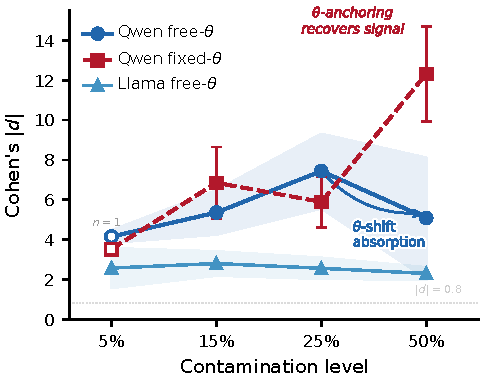
\includegraphics[width=\columnwidth]{fig_dose_response.pdf}
  \caption{Dose-response trajectories on MMLU. Free-$\theta$ (solid) shows non-monotonic behavior for Qwen due to $\theta$-shift absorption (shaded); fixed-$\theta$ (dashed) removes the inverted-U artifact and yields an overall positive dose-response ($|d|{=}12.32$ at 50\%). Llama's flat trajectory reflects minimal absorption. Hollow markers: single-seed ($n{=}1$); error bars: $\pm$SD ($n{=}3$).}
  \label{fig:dose_response}
\end{figure}

\subsection{$\Delta\ell_z^*$ Matched-Difference Design}
\label{sec:did}

LLM response patterns systematically violate IRT assumptions of local independence and unidimensionality.
In our empirical data, 57 of 60 model-benchmark cells yield $|\ell_z^*| > 1.96$ even absent contamination, rendering absolute thresholds uninformative.
We address this through a matched-difference design.

For controlled experiments with clean baselines, we compute:
\begin{equation}
  \Delta\ell_z^* = \ell_{z,\text{contam}}^{*} - \bar{\ell}_{z,\text{clean}}^{*}
  \label{eq:delta_lz}
\end{equation}
where $\bar{\ell}_{z,\text{clean}}^{*}$ averages over $n{=}10$ clean seeds.
The shared model misfit cancels, isolating contamination-specific aberrance.
We quantify effect sizes as $d = (\ell_{z,\text{contam}}^{*} - \bar{\ell}_{z,\text{clean}}^{*})\,/\,s_{\text{clean}}$, where $s_{\text{clean}}$ is the SD of the $n{=}10$ clean-seed $\ell_z^*$ values; with a single contaminated observation per condition, $d$ is a standardized departure rather than a two-sample effect size (Hedges' $g = J \cdot d$, $J \approx 0.914$ for $n{=}10$; \citealp{hedges1981}).
We report percentile bootstrap 95\% CIs (10,000 resamples) reflecting clean-seed variability only; bias-corrected and accelerated (BCa) correction (Appendix~\ref{app:bca}) generally confirms conservative coverage; multi-seed contamination-run variance appears in Appendix~\ref{app:reproducibility}.

For deployment without clean baselines, cross-benchmark comparison provides the reference: the target benchmark's $\ell_z^*$ is compared against benchmarks presumed clean from the same model.
Significance thresholds derive from a nonparametric bootstrap null rather than the asymptotic $\mathcal{N}(0,1)$ reference, accommodating residual model misspecification.
Simulation analysis (Appendix~\ref{app:local_dep}) confirms that the matched-difference design is robust to local dependence at realistic levels ($d_{\text{ratio}} \geq 0.93$ for $\sigma_\tau \leq 0.5$) and maintains ${\geq}98.5\%$ power even under contamination-specific asymmetric dependence.

\subsection{Experimental Setup}
\label{sec:setup}

\paragraph{Models and contamination.}
We validate on three 7--8B model families: Qwen2.5-7B-Instruct, Llama-3.1-8B-Instruct, and Mistral-7B-Instruct-v0.3.
Each is fine-tuned with Quantized Low-Rank Adaptation (QLoRA; rank\,$=$\,16, $\alpha$\,$=$\,32; full hyperparameters in Appendix~\ref{app:hyperparams}) under clean and contaminated conditions at varying levels: at $X\%$ contamination, $X\%$ of SFT training examples are benchmark items (questions paired with gold answers in the standard evaluation format), with the remainder drawn from a general instruction-following dataset.
All three families are tested at 15\% and 50\% contamination.
Following initial observation of non-monotonic dose-response for Qwen, we added 5\% and 25\% conditions for Qwen to trace the full dose-response curve.
Both conditions were subsequently extended to Llama to test whether the pattern generalizes; Mistral was additionally tested at 5\% but not at 25\% due to computational constraints.
We train $n{=}10$ independent clean seeds per model to establish baseline variability and construct bootstrap confidence intervals.
Reported CIs reflect variability across $n$ clean baseline seeds; for each model family, selected contamination levels were additionally replicated with $n{=}3$ independent QLoRA seeds to assess training-run variance: Qwen at 15\%/25\%/50\%, Llama at 5\%/15\%/25\%/50\%, and Mistral at 5\%/15\%/50\% (Appendix~\ref{app:reproducibility}).

\paragraph{Benchmarks.}
We evaluate on MMLU \citep{hendrycks2021mmlu} (14,042 items) and ARC-Challenge \citep{clark2018arc} (295 PSN-IRT-calibrated items), spanning two orders of magnitude in benchmark size.
All 4PL item parameters are from \citet{psnirt2026}.
ARC-Challenge experiments were conducted on Qwen only, as the primary evaluation of cross-benchmark generalizability; extending to additional families was constrained by computational budget.

\paragraph{Post-RL extension.}
To probe behavior boundaries beyond SFT, we apply Group Relative Policy Optimization (GRPO; \citealp{shao2024}) to one contaminated Qwen model (15\% MMLU) for 1,500 steps, evaluating at three checkpoints.
This extension is $N{=}1$ (single model family, single contamination level).

\paragraph{Evaluation protocol.}
Ability estimation uses maximum likelihood (MLE) with Newton--Raphson optimization on the 4PL log-likelihood.
For each model, we compute $\ell_z^*$ on the full benchmark response vector; seen/unseen decomposition recomputes $\ell_z^*$ on item subsets to localize the contamination signal.
All evaluations use greedy decoding (temperature~0) with the standard multiple-choice prompt format from the lm-evaluation-harness \citep{eval-harness}.

\paragraph{Contamination model.}
QLoRA SFT on benchmark items proxies SFT-stage contamination, analogous to a test-taker with item preknowledge.
At each contamination level, contaminated items are shuffled into the training mixture and presented in the same question--answer format used during evaluation, maximizing the memorization signal.
We term contaminated items \emph{seen} and the remainder \emph{unseen}, enabling person-fit decomposition (\S\ref{sec:degradation}).
Findings are scoped to SFT-based contamination.

\section{Results}
\label{sec:results}

\begin{table}[t]
\centering
\caption{Cohen's $d$ for $\Delta\ell_z^*$ across model families ($n{=}10$ clean seeds). Single-seed conditions: percentile bootstrap 95\% CI (10,000 resamples). $^{\dagger}$Multi-seed conditions: mean $\pm$ SD ($n{=}3$ independent runs). All single-seed CIs exclude zero.}
\label{tab:cohens_d}
\footnotesize
\resizebox{\columnwidth}{!}{%
\begin{tabular}{@{}llrrrr@{}}
\toprule
Model & Bench. & $d$ (5\%) [CI] & $d$ (15\%) [CI] & $d$ (25\%) [CI] & $d$ (50\%) [CI] \\
\midrule
Qwen$^{\dagger}$ & MMLU & $-4.15$ [$-9.9$, $-2.7$] & $-5.36$ ($\pm$1.10) & $-7.44$ ($\pm$1.86) & $-5.08$ ($\pm$3.02) \\
Llama$^{\dagger}$ & MMLU & $-2.57$ ($\pm$0.99) & $-2.80$ ($\pm$0.60) & $-2.56$ ($\pm$0.52) & $-2.30$ ($\pm$0.30) \\
Mistral$^{\dagger}$ & MMLU & $-3.83^{*}$ ($\pm$1.42) & $-3.37$ ($\pm$0.68) & --- & $-4.09$ ($\pm$0.53) \\
Qwen$^{\dagger}$ & ARC-C & --- & $+3.16$ [$2.0$, $9.5$] & --- & $+5.30$ [$3.6$, $15.2$] \\
\bottomrule
\multicolumn{6}{@{}l}{\scriptsize $^{\dagger}$Multi-seed conditions: means ($n{=}3$ independent runs) shown as $\pm$SD; remaining conditions are single-seed with bootstrap CIs.} \\
\multicolumn{6}{@{}l}{\scriptsize $^{*}$$n{=}2$ seeds. Per-seed values in Appendix~\ref{app:reproducibility}.}
\end{tabular}}
\end{table}

\subsection{Detection Signal Across Model Families}
\label{sec:detection}

Table~\ref{tab:cohens_d} presents Cohen's $d$ effect sizes for $\ell_z^*$ across three model families and two benchmarks.
All single-seed bootstrap CIs exclude zero, confirming that $\Delta\ell_z^*$ reliably separates contaminated from clean models at both contamination levels.

On MMLU, effect sizes range from $|d|{=}2.30$ (Llama at 50\%) to $|d|{=}7.44$ (Qwen at 25\%), with Qwen at 5\% ($|d|{=}4.15$) confirming detection at the lowest contamination level tested. Llama ($|d|{=}2.57$/$2.80$/$2.56$/$2.30$) and Mistral ($|d|{=}3.83$/$3.37$/$4.09$) show comparable magnitudes.
On ARC-C (295 items), Qwen yields $|d|{=}3.16$ at 15\% and $|d|{=}5.30$ at 50\%, demonstrating that detection remains feasible even on small benchmarks when contamination is sufficiently concentrated.
The positive sign on ARC-C (vs.\ negative on MMLU) reflects a ceiling effect: with 89.7\% baseline accuracy, contamination pushes responses toward over-consistency rather than the unexpected-success pattern seen on MMLU.

Clean-model $\ell_z^*$ baselines diverge substantially: Qwen ${+}8.68$ (over-consistent), Llama ${-}0.14$ (near-expected), Mistral ${+}4.02$ (Appendix~\ref{app:baseline_meaning}); seed sensitivity analysis confirms these reflect systematic misfit rather than seed artifacts (Appendix~\ref{app:seed_sensitivity}), making absolute thresholds uninformative.
The $\Delta\ell_z^*$ design normalizes these divergent baselines (Figure~\ref{fig:heatmap}).

\begin{figure}[t]
  \centering
  
\includegraphics[width=\columnwidth]{fig_heatmap.pdf}
  \caption{Cohen's $|d|$ heatmap (values from Table~\ref{tab:cohens_d}; multi-seed means where available). Blue intensity reflects effect-size magnitude. Grey cells: not tested.}
  \label{fig:heatmap}
\end{figure}

\subsection{Model-Specific $\theta$-Shift Dynamics}
\label{sec:theta_dynamics}

Contamination inflates $\hat{\theta}_{\text{MLE}}$, which ``explains away'' anomalous successes on hard items; we term this \emph{$\theta$-shift absorption}.
$\theta$-shift magnitude is comparable across families ($\Delta\theta{\approx}0.5$), yet fixed-$\theta$ amplification diverges markedly (Table~\ref{tab:theta_fixed}; Figure~\ref{fig:composite}c).

$\theta$-shift absorption is the dominant source of detection variability for high-ability models at high contamination:
(i) fixed-$\theta$ estimation amplifies Qwen's multi-seed $|d|$ by 2.4$\times$ at 50\% ($5.08 \to 12.32$; Table~\ref{tab:theta_fixed}), while Llama shows no amplification ($0.4\times$);
(ii) $\theta$-anchoring reduces Qwen's inter-seed CV from 60\% to 19\%, confirming that training-run variance is driven by $\theta$-shift stochasticity rather than true signal variance;
(iii) the cross-model ranking under free-$\theta$ is seed-dependent at 50\%, making $\theta$-anchoring a necessary condition for reliable detection of high-ability models at high contamination.

ARC-C reverses this pattern: despite 89.7\% baseline accuracy, contamination produces \emph{larger} effect sizes ($|d|{=}3.16$/$5.30$).
This ceiling effect arises because 295 items with high baseline accuracy leave minimal room for $\theta$ inflation; contamination manifests as anomalous successes on the few remaining hard items, producing disproportionately large $\ell_z^*$ shifts.
Detection sensitivity thus depends on the interaction between model ability and benchmark characteristics, suggesting that practitioners should interpret effect sizes relative to the specific model--benchmark pairing rather than applying universal thresholds.

\paragraph{Seen vs.\ unseen decomposition.}
To localize the contamination signal, we recompute $\ell_z^*$ separately on seen and unseen item subsets.
At 15\% contamination, Qwen's seen-item $\ell_z^*$ drops to $+0.67$ while unseen items remain at $+3.91$ (seed 42; clean baseline $+8.68$), confirming that the person-fit signal originates predominantly from memorized items.
This decomposition is unique to $\ell_z^*$ among the statistics we evaluate: neither accuracy $z$-scores nor HT support item-subset analysis.

\paragraph{Fixed-$\theta$ estimation.}
Table~\ref{tab:theta_fixed} compares free- and fixed-$\theta$ Cohen's $d$.
The amplification ratio tracks baseline $|\ell_z^*|$ monotonically: Qwen ($\ell_z^*{=}{+}8.68$) shows $2.4{\times}$ at 50\%, Mistral ($+4.02$) $1.7{\times}$, while Llama ($-0.14$) shows $0.4{\times}$ despite comparable $\theta$-shift ($\Delta\theta{=}0.52$).
Fixed-$\theta$ is thus a targeted remedy for models with substantial baseline misfit, not a universal one.

\begin{table}[t]
\centering
\caption{Free-$\theta$ vs.\ fixed-$\theta$ Cohen's $|d|$ on MMLU. Qwen$^{\S}$: multi-seed mean ($n{=}3$); Llama and Mistral: seed-42 single run. Fixed-$\theta$ anchors $\hat{\theta}$ at the clean-model mean, eliminating $\theta$-shift absorption.}
\label{tab:theta_fixed}
\footnotesize
\resizebox{\columnwidth}{!}{%
\begin{tabular}{@{}lcccc@{}}
\toprule
Model & $|d_{\text{free}}|$ & $|d_{\text{fixed}}|$ & Ratio & Fixed 95\% CI / SD \\
\midrule
\multicolumn{5}{@{}l}{\textit{5\% contamination}} \\
Qwen & 4.15 & 3.52 & 0.8$\times$ & [2.9, 5.7] \\
\addlinespace
\multicolumn{5}{@{}l}{\textit{15\% contamination}} \\
Qwen$^{\S}$ & 5.36 & 6.85 & 1.3$\times$ & ($\pm$1.80) \\
Llama & 2.11 & 0.58 & 0.3$\times$ & [0, 2.37]$^{\dagger}$ \\
Mistral$^{\ddagger}$ & 2.64 & 2.69 & 1.0$\times$ & [1.53, 9.06] \\
\addlinespace
\multicolumn{5}{@{}l}{\textit{50\% contamination}} \\
Qwen$^{\S}$ & 5.08 & 12.32 & 2.4$\times$ & ($\pm$2.38) \\
Llama & 2.33 & 0.84 & 0.4$\times$ & [0.17, 2.97] \\
Mistral$^{\ddagger}$ & 3.50 & 5.80 & 1.7$\times$ & [3.87, 18.45] \\
\bottomrule
\multicolumn{5}{@{}l}{\scriptsize $^{\dagger}$CI includes zero.} \\
\multicolumn{5}{@{}l}{\scriptsize $^{\S}$Multi-seed mean ($n{=}3$); CI column shows $\pm$SD of fixed-$\theta$ $|d|$.} \\
\multicolumn{5}{@{}l}{\scriptsize $^{\ddagger}$Fixed-$\theta$: 6 seeds (response vectors from seeds 4--7 excluded due to incomplete evaluation runs); free-$\theta$ uses all 10.} \\
\multicolumn{5}{@{}p{0.9\columnwidth}}{\scriptsize $d_{\text{free}}$ CIs omitted; multi-seed means in Table~\ref{tab:cohens_d}.}
\end{tabular}}
\end{table}

\subsection{Detection-Diagnosis Tradeoff}
\label{sec:degradation}

Table~\ref{tab:degradation} compares three statistics: $\ell_z^*$ (4PL parameters), HT (difficulty only), and accuracy $z$-scores (no item parameters).
For pure detection, simpler statistics are more powerful: accuracy $z$-scores yield $|d|$ values up to an order of magnitude larger than person-fit statistics, because cross-seed accuracy variance is near-zero ($\text{SD}{\approx}0.0003$ for Qwen clean seeds).
These extreme effect sizes reflect the controlled setting where training-run variance is minimal; in deployment without matched clean baselines, accuracy $z$-scores would lack this stability.
HT generally exceeds $\ell_z^*$, since HT is not attenuated by the Snijders correction.

Yet the diagnostic power reverses.
$\ell_z^*$ uniquely supports (a)~\emph{seen/unseen decomposition}, though item-level detection is near-random (area under the ROC curve [AUROC]\,${\approx}\,0.53$; Appendix~\ref{app:item_auroc}); (b)~\emph{$\theta$-shift mechanism} (\S\ref{sec:theta_dynamics}); and (c)~\emph{structural sensitivity}: $\ell_z^*$ flags 57/60 leaderboard cells as aberrant (Figure~\ref{fig:leaderboard_heatmap}) vs.\ 4/60 for accuracy $z$-scores \citep{stonge2011}.
In practice, accuracy $z$-scores screen candidates; $\ell_z^*$ then characterizes whether the signal reflects $\theta$-shift absorption or direct memorization.
Within the IRT family, 4PL gains $+$55.7pp power over 3PL on MMLU at 15\% contamination ($96.9\%$ vs.\ $41.2\%$; Appendix~\ref{app:4pl_ablation}), because 46\% of MMLU items have upper asymptote $d < 0.95$; the advantage persists across benchmarks (HellaSwag $+$34.3pp, GSM8K $+$20.7pp).

\begin{table}[t]
\centering
\caption{Detection-diagnosis tradeoff on MMLU: Cohen's $|d|$ across three statistics. Qwen$^\dagger$: multi-seed means ($n{=}3$); Llama and Mistral: seed-42 single run with bootstrap CIs.}
\label{tab:degradation}
\footnotesize
\begin{tabular}{@{}llrr@{}}
\toprule
Model & Statistic & $|d|$ (15\%) & $|d|$ (50\%) \\
\midrule
Qwen$^\dagger$ & $\ell_z^*$ & $5.36$ ($\pm$1.10) & $5.08$ ($\pm$3.02) \\
     & HT & $5.83$ ($\pm$1.30) & $5.29$ ($\pm$3.41) \\
     & Acc.\ $z$ & $45.0$ ($\pm$2.5) & $70.0$ ($\pm$1.1) \\
\addlinespace
Llama & $\ell_z^*$ & $2.11$ [$1.4$, $4.8$] & $2.33$ [$1.6$, $5.1$] \\
      & HT & $2.45$ [$1.5$, $4.3$] & $3.07$ [$1.9$, $5.3$] \\
      & Acc.\ $z$ & $22.5$ [$13.6$, $47.0$] & $32.8$ [$19.8$, $68.6$] \\
\addlinespace
Mistral & $\ell_z^*$ & $2.64^{\ddagger}$ & $3.50$ [$2.1$, $9.4$] \\
      & HT & $4.36$ [$1.2$, $7.0$] & $5.89$ [$1.9$, $9.4$] \\
      & Acc.\ $z$ & $7.81$ [$4.4$, $14.4$] & $16.6$ [$9.7$, $34.6$] \\
\bottomrule
\multicolumn{4}{@{}p{0.9\columnwidth}}{\scriptsize $^\dagger$Per-seed values in Appendix~\ref{app:reproducibility}. Bootstrap CIs: 10{,}000 resamples over $n{=}10$ clean seeds. $^{\ddagger}$Seed-42 single run; multi-seed $|d|{=}3.37$ ($\pm$0.68) in Table~\ref{tab:cohens_d}.}
\end{tabular}
\end{table}

\begin{figure}[t]
  \centering
  
\includegraphics[width=\columnwidth]{fig_4_model_heatmap.pdf}
  \caption{$\ell_z^*$ heatmap for 12 leaderboard models across five benchmarks. 57/60 cells exceed $|\ell_z^*| > 1.96$, indicating pervasive IRT assumption violations even absent contamination. Details in Appendix~\ref{app:leaderboard_aberrance}.}
  \label{fig:leaderboard_heatmap}
\end{figure}

\subsection{Ability-Dependent Non-Monotonic Dose-Response}
\label{sec:inverted_u}

As an exploratory observation, the free-$\theta$ dose-response is non-monotonic for Qwen.
Figure~\ref{fig:dose_response} plots the dose-response trajectory, combining the single-seed 5\% estimate (hollow marker) with multi-seed means at 15\%/25\%/50\% ($|d|$: $4.15 \to 5.36 \to 7.44 \to 5.08$), showing signal peaking at 25\% before declining; inter-seed variance at 50\% is high (CV${=}$60\%, range $[1.90, 7.91]$).
This non-monotonicity is a $\theta$-estimation artifact: fixed-$\theta$ eliminates the inverted-U ($|d|{=}12.32$ at 50\%, CV reduced to 19\%).
Llama's flat trajectory ($|d|{\approx}2.3$--$2.8$) is consistent with its near-zero baseline $\ell_z^*$: the divergence is fully explained by baseline ability differences.
Simulation corroborates: two-sided testing achieves ${>}$93\% power at all levels on MMLU (Appendix~\ref{app:simulation}).
These results demonstrate that non-monotonic dose-response is not a fundamental limitation of person-fit statistics but a predictable consequence of free-$\theta$ estimation in high-ability models, and that $\theta$-anchoring provides a principled correction.

\section{Discussion}\label{sec:discussion}

Our findings reveal both the strengths and boundaries of IRT person-fit for contamination detection: $\ell_z^*$ reliably detects SFT-stage contamination across model families, but three boundary conditions constrain its practical utility.

\paragraph{Characterization over tool.}
The detection-diagnosis tradeoff (\S\ref{sec:degradation}) shows that simpler statistics detect contamination more powerfully than $\ell_z^*$: accuracy $z$-scores yield $|d|$ values several-fold to over an order of magnitude larger, and HT generally exceeds $\ell_z^*$.
The value of the IRT framework lies not in detection power but in mechanistic understanding: the $\theta$-shift analysis reveals \emph{why} detection sensitivity varies across models and contamination levels, the seen/unseen decomposition identifies \emph{what fraction} of items are memorized, and the 4PL parameterization captures item-level ceiling effects that 3PL misattributes as aberrance.
These diagnostics are invisible to accuracy $z$-scores or HT; our contribution lies in quantifying these theoretically predictable effects in the LLM setting, where magnitudes and boundary conditions are not derivable from theory alone.

\paragraph{Practical implications.}
Two results have immediate consequences.
Free-$\theta$ estimation produces seed-dependent dose-response curves (CV up to 60\%); $\theta$-anchoring stabilizes detection for models whose clean $\ell_z^*$ departs substantially from zero.
$\ell_z^*$ is most informative for large benchmarks ($n \approx 8{,}000$ items for 80\% power at 15\% contamination); on small benchmarks like ARC-C, detection relies on concentrated contamination effects.

\paragraph{Scope and calibration.}
Universal baseline misfit (57/60 cells flagged) confirms systematic IRT violations; the $\Delta\ell_z^*$ design turns this into a feature through within-model differencing.
PSN-IRT provides pre-calibrated 4PL parameters \citep{psnirt2026}, but classical calibration fails on contaminated data ($r_a{=}0.127$; Appendix~\ref{app:mml_em}); the robustness analysis (Appendix~\ref{app:param_perturb}) provides partial reassurance (${\pm}10\%$ noise tolerance).
\paragraph{Information requirements and method positioning.}
$\ell_z^*$ sits below MIA \citep[logits;][]{minkprob2024} and ConStat \citep[multi-benchmark scores;][]{constat2024} in an information-requirements hierarchy, needing only single-benchmark binary patterns and an external item bank---suited to retrospective audits where logits are unavailable. Our GRPO pilot confirms this: Min-K\% AUC drops to chance ($0.493$) post-RL while $\ell_z^*$ signal persists (${\sim}3.3$; Figure~\ref{fig:grpo}), consistent with \citet{wang2025fragility}.

\section{Conclusion}\label{sec:conclusion}

We characterized IRT person-fit statistics for LLM contamination detection across three 7--8B model families, establishing reliable SFT-stage detection while identifying boundary conditions: $\theta$-shift absorption necessitating $\theta$-anchored estimation for high-ability models, a detection-diagnosis tradeoff, and non-monotonic dose-response as a $\theta$-estimation artifact.
For practitioners, we recommend a two-stage workflow: accuracy $z$-scores for efficient screening, followed by $\ell_z^*$ analysis when mechanistic understanding is needed---distinguishing \emph{which} items drive aberrance rather than merely flagging contamination.
Beyond detection, person-fit statistics capture response-pattern anomalies that persist after RL post-training erases memorization-based signals, complementing logit-based methods.
Future work should address pretraining-stage signatures, broader model scales, and cross-benchmark generalization with larger item banks.


\section*{Limitations}

Our controlled experiments cover three 7--8B model families with QLoRA fine-tuning; generalization to larger scales, mixture-of-experts architectures, full-parameter fine-tuning, and pretraining-stage contamination remains untested.
Most contamination conditions use a single training run, and multi-seed replication (available for Qwen) reveals high seed dependence at 50\% contamination (CV${=}$60\%), partially resolved by $\theta$-anchoring; the post-RL characterization is $N{=}1$.
The framework depends on pre-calibrated 4PL item parameters from PSN-IRT, whose calibration sample may include contaminated models, and we do not provide head-to-head comparison with logit-based methods (MIA, ConStat) that operate at a different information level.


\section*{Reproducibility Statement}
Code and response data will be released upon acceptance.
Bootstrap confidence intervals use the percentile method with 10,000 resamples.
All three model families use clean baseline seeds 0--9 ($n{=}10$ per family).
Pre-calibrated 4PL item parameters are from the publicly available PSN-IRT item bank \citep{psnirt2026}.
Training used PyTorch 2.8.0, Transformers 5.8.1, PEFT 0.19.1, and BitsAndBytes 0.49.2.
Both benchmarks are publicly available under permissive licenses (MMLU: MIT; ARC-Challenge: CC-BY-SA).

\bibliography{references}

\appendix
\section{Simulation Validation}
\label{app:simulation}

Under the null (no contamination), bootstrap $\ell_z^*$ tracks $\mathcal{N}(0,1)$: mean bias 0.041 and standard deviation 1.003 on MMLU.
Kolmogorov--Smirnov rejection rates vary with benchmark size: 8.3\% for MMLU and HellaSwag ($n > 10{,}000$), 50.0\% for GSM8K ($n = 1{,}319$), 58.3\% for ARC-C ($n = 295$), and 75.0\% for HumanEval ($n = 164$).
$\ell_z^*$ is well-calibrated for benchmarks with $n \geq 10{,}000$ items; smaller benchmarks show increasing finite-sample deviations from normality.

Two-sided testing eliminates the inverted-U artifact: MMLU achieves 97.8\% power at 15\% contamination and sustains ${>}$93\% at all levels.
Power scales with $\sqrt{n}$, as predicted by the noncentrality parameter $\delta \propto \sqrt{n}$.
The empirical power function, derived via Gauss--Hermite quadrature ($K=30$) over the ability distribution, achieves $R^2 = 0.957$ against simulated values, with approximate minimum benchmark size of $n \geq 7{,}958$ items for 80\% power at 15\% contamination under MMLU item parameters.

\section{4PL vs.\ 3PL Ablation Details}
\label{app:4pl_ablation}

Table~\ref{tab:4pl_3pl_power} reports detection power (proportion of 2{,}000 simulation replicates rejecting $H_0$ at $\alpha{=}0.05$, two-sided) for 4PL and 3PL parameterizations across five benchmarks and seven contamination levels.
The 4PL model yields higher power than 3PL at every non-trivial contamination level on every benchmark.
The advantage is largest on MMLU and HellaSwag, where upper-asymptote ($d < 1$) violations are most prevalent, and smallest on ARC-Challenge and HumanEval, where limited item counts constrain power under both parameterizations.

Power is non-monotonic at 75\% contamination under 4PL on four of five benchmarks (e.g., MMLU: $.952 \to .938$; GSM8K: $.846 \to .802$).
This reflects the $\theta$-shift boundary condition described in \S\ref{sec:inverted_u}: at high contamination fractions, re-estimated $\hat{\theta}$ absorbs part of the aberrance signal, reducing $|\ell_z^*|$.
At 100\% contamination, all items are seen and power reaches 1.000 trivially.
The 4PL advantage over 3PL depends on accurate estimation of the upper asymptote $d$; with estimation error exceeding ${\sim}10\%$, the effective model behavior approaches 3PL ($d{=}1$) and the power gain diminishes.
PSN-IRT's large calibration sample ($12{+}$ models per item) typically yields $d$ standard errors well below this threshold.

\begin{table*}[t]
\centering
\caption{Detection power (proportion rejecting $H_0$ at $\alpha{=}0.05$) under 4PL and 3PL parameterizations across benchmarks and contamination levels ($n{=}2{,}000$ replicates per cell). Bold indicates the 4PL advantage exceeds 5\,pp.}
\label{tab:4pl_3pl_power}
\small
\begin{tabular}{@{}llccccccc@{}}
\toprule
Benchmark & IRT & 5\% & 10\% & 15\% & 25\% & 50\% & 75\% & 100\% \\
\midrule
MMLU & 4PL & \textbf{.476} & \textbf{.848} & \textbf{.969} & \textbf{.983} & \textbf{.952} & \textbf{.938} & 1.00 \\
     & 3PL & .227 & .340 & .412 & .521 & .676 & .770 & 1.00 \\
\addlinespace
HellaSwag & 4PL & \textbf{.251} & \textbf{.454} & \textbf{.656} & \textbf{.915} & \textbf{.939} & \textbf{.919} & 1.00 \\
          & 3PL & .167 & .241 & .313 & .368 & .508 & .642 & 1.00 \\
\addlinespace
GSM8K & 4PL & \textbf{.156} & \textbf{.309} & \textbf{.492} & \textbf{.737} & \textbf{.846} & \textbf{.802} & 1.00 \\
      & 3PL & .102 & .172 & .285 & .396 & .567 & .577 & 1.00 \\
\addlinespace
ARC-C & 4PL & .057 & .075 & .087 & \textbf{.130} & \textbf{.285} & \textbf{.493} & 1.00 \\
      & 3PL & .054 & .062 & .071 & .076 & .110 & .102 & 1.00 \\
\addlinespace
HumanEval & 4PL & .076 & .121 & \textbf{.197} & \textbf{.302} & \textbf{.554} & \textbf{.521} & 1.00 \\
          & 3PL & .063 & .086 & .120 & .182 & .281 & .315 & 1.00 \\
\bottomrule
\end{tabular}
\end{table*}

\section{Seed Sensitivity Analysis}
\label{app:seed_sensitivity}

\paragraph{Clean-baseline variability.}
Table~\ref{tab:seed_sensitivity} reports $\ell_z^*$, accuracy, and $\hat{\theta}_{\text{MLE}}$ across three independent QLoRA runs (seeds 42, 123, 456).
For Qwen2.5-7B, $\ell_z^*$ ranges from $7.05$ (seed 123) to $9.53$ (seed 456); the lower value of seed 123 likely reflects seed-specific training dynamics (random initialization, data ordering), but all three seeds produce $\ell_z^* \gg 1.96$, confirming that the elevated baseline reflects systematic model--benchmark misfit rather than seed-specific artifacts.
Llama-3.1-8B shows $\ell_z^*$ near zero ($-0.14 \pm 0.97$), consistent with lower baseline misfit.
Accuracy variability is negligible for both families (CV $< 0.004$).

\begin{table}[t]
\centering
\caption{Seed sensitivity analysis for clean baseline across three independent runs (seeds 42, 123, 456). CV = coefficient of variation ($\mathrm{std}/|\mathrm{mean}|$). These $n{=}3$ pilot results are superseded by the $n{=}10$ analysis in \S\ref{sec:detection}; retained for methodological transparency.}
\label{tab:seed_sensitivity}
\footnotesize
\resizebox{\columnwidth}{!}{%
\begin{tabular}{@{}llcccc@{}}
\toprule
Model & Metric & Mean & Std & Range & CV \\
\midrule
Qwen2.5-7B & $\ell_z^*$ & 8.684 & 1.412 & 2.475 & 0.163 \\
 & Accuracy & 0.679 & 0.000 & 0.001 & 0.001 \\
 & $\hat{\theta}_{\mathrm{MLE}}$ & $-$0.097 & 0.012 & 0.023 & 0.119 \\
\midrule
Llama-3.1-8B & $\ell_z^*$ & $-$0.141 & 0.965 & 1.929 & 6.860 \\
 & Accuracy & 0.594 & 0.002 & 0.004 & 0.004 \\
 & $\hat{\theta}_{\mathrm{MLE}}$ & $-$0.645 & 0.019 & 0.036 & 0.029 \\
\bottomrule
\end{tabular}}
\end{table}

\paragraph{Cohen's $d$ confidence intervals.}
Table~\ref{tab:cohens_d_ci} reports Cohen's $d$ effect sizes with both analytic and bootstrap 95\% confidence intervals.
Analytic CIs use $d \pm t_{0.025,\,\text{df}=2} \cdot \text{SE}_d$; with only $n{=}3$ clean seeds (df${=}2$), the critical value $t_{0.025,2} = 4.303$ produces intervals wide enough to cross zero in all four conditions.
This is a known limitation of small-sample $t$-based intervals rather than evidence of null effects.
Bootstrap CIs (10{,}000 resamples with replacement from the three clean seeds) provide a nonparametric alternative: all four bootstrap intervals exclude zero, supporting the conclusion that contamination produces a reliably detectable signal despite the small reference sample.

\begin{table}[t]
\centering
\caption{Cohen's $d$ with 95\% confidence intervals for contaminated conditions relative to clean baselines ($n{=}3$ seeds). Analytic CIs use $t_{0.025, \text{df}=2}$; bootstrap CIs use 10{,}000 resamples. These $n{=}3$ pilot results are superseded by the $n{=}10$ analysis in \S\ref{sec:detection}; retained for methodological transparency.}
\label{tab:cohens_d_ci}
\footnotesize
\resizebox{\columnwidth}{!}{%
\begin{tabular}{@{}llccc@{}}
\toprule
Model & Cond. & $d$ & Analytic CI & Bootstrap CI \\
\midrule
Qwen & 15\% & $-$3.42 & [$-$9.92, 3.08] & [$-$3.45, $-$2.82] \\
 & 50\% & $-$0.99 & [$-$4.02, 2.04] & [$-$0.99, $-$0.41] \\
\midrule
Llama & 15\% & $-$2.95 & [$-$8.70, 2.80] & [$-$5.89, $-$2.29] \\
 & 50\% & $-$3.31 & [$-$9.63, 3.01] & [$-$6.47, $-$2.59] \\
\bottomrule
\end{tabular}}
\end{table}

\paragraph{Cross-family consistency.}
Table~\ref{tab:cross_family} confirms that both model families produce large negative Cohen's $d$ under contamination.
The $|\Delta d| = 2.32$ gap at 50\% contamination reflects Qwen's non-monotonic dose-response (the $\theta$-shift boundary condition; \S\ref{sec:inverted_u}), not a failure of detection robustness---both families remain well above conventional large-effect thresholds ($|d| > 0.8$) at both contamination levels.

\begin{table}[t]
\centering
\caption{Cross-family consistency of contamination detection ($n{=}3$ pilot). Both families show large negative $d$ under contamination. Superseded by $n{=}10$ results in \S\ref{sec:detection}; retained for methodological transparency.}
\label{tab:cross_family}
\small
\begin{tabular}{@{}lcccl@{}}
\toprule
Condition & Qwen $d$ & Llama $d$ & $|\Delta d|$ & Consistent? \\
\midrule
15\% contam. & $-$3.42 & $-$2.95 & 0.47 & Yes \\
50\% contam. & $-$0.99 & $-$3.31 & 2.32 & Yes \\
\bottomrule
\end{tabular}
\end{table}

\section{Baseline $\ell_z^*$ Interpretation}
\label{app:baseline_meaning}

The baseline $\ell_z^*$ value reflects a model's difficulty-ordering consistency under the 4PL model, not its accuracy alone.
In the PSN-IRT leaderboard data (12 models $\times$ 5 benchmarks), Mistral ($\text{acc}{=}0.514$, lowest among the 12 models) exhibits $\ell_z^*{=}{+}5.42$ (second highest), because its response pattern follows the IRT-predicted difficulty ordering more closely than higher-accuracy models whose responses violate the assumed item structure.
This dissociation explains why Mistral produces the strongest contamination signal despite the lowest accuracy: its lower baseline ability ($\hat{\theta}{=}{-}1.16$) provides greater $\theta$-shift headroom.

\section{Leaderboard Aberrance Analysis}
\label{app:leaderboard_aberrance}

We computed $\ell_z^*$ and accuracy $z$-scores for all 12 models $\times$ 5 benchmarks $=$ 60 cells in the PSN-IRT leaderboard dataset.
Using the standard $|\ell_z^*| > 1.96$ threshold ($\alpha{=}0.05$, two-tailed), 57 of 60 cells are flagged as aberrant, indicating pervasive IRT assumption violations in production LLM responses.
In contrast, accuracy $z$-scores ($|z| > 1.96$) flag only 4 of 60 cells.
This stark asymmetry---95\% aberrance by $\ell_z^*$ versus 7\% by accuracy---motivates the $\Delta\ell_z^*$ matched-difference design (\S\ref{sec:did}), which sidesteps absolute thresholds by comparing each model against its own clean baseline.

\section{Item-Level Detection Results}
\label{app:item_auroc}

Table~\ref{tab:item_auroc} reports item-level contamination detection performance at 15\% contamination on MMLU.
All methods perform near random (AUROC $\leq 0.63$), confirming that contamination is diffuse across the response pattern and that model-level aggregation via $\ell_z^*$ is essential.

An accuracy $z$-score baseline yields $z{=}160$ at 15\% contamination, but this reflects near-zero cross-seed accuracy variance ($\text{std}{=}0.0003$), not genuine discriminability.
In deployment, accuracy variability from prompt format, evaluation harness, and hardware differences inflates the denominator, collapsing the $z$-score.

\begin{table}[t]
\centering
\caption{Item-level contamination detection (AUROC) at 15\% contamination on MMLU.}
\label{tab:item_auroc}
\footnotesize
\begin{tabular}{@{}lc@{}}
\toprule
Method & AUROC \\
\midrule
Random baseline & 0.50 \\
$\ell_z^*$ itemwise & 0.53 \\
LR cross-model & 0.59 \\
RF cross-model & 0.63 \\
\bottomrule
\end{tabular}
\end{table}

\section{Robustness Analysis}
\label{app:robustness}

\subsection{$\Delta\ell_z^*$ Under Local Dependence}
\label{app:local_dep}

IRT person-fit statistics assume local independence---conditional on $\theta$, item responses are independent.
LLM benchmarks violate this assumption through topical clustering (e.g., MMLU subjects); resampling-based approaches can provide valid person-fit assessment even under such violations \citep{sinharay2016}.
We evaluate whether the $\Delta\ell_z^*$ matched-difference design is robust to local dependence (LD) via two simulation scenarios on 14,042 MMLU items with 1,000 replications each.

\paragraph{Shared LD.}
Clean and contaminated conditions share identical testlet structure (${\sim}200$ testlets of ${\sim}70$ items, random effect $\gamma_t \sim \mathcal{N}(0, \sigma_\tau)$).
Table~\ref{tab:ld_shared} reports absolute $\ell_z^*$ Type~I error and the ratio of $\Delta\ell_z^*$ effect size ($d$) to the no-LD baseline.
While absolute $\ell_z^*$ Type~I error inflates severely under LD (0.043$\to$0.939 at $\sigma{=}1.0$), the $\Delta\ell_z^*$ design maintains detection power: $d_{\text{ratio}} \geq 0.93$ for $\sigma_\tau \leq 0.5$ (realistic range), confirming that shared misfit is cancelled by the matched-difference design.

\begin{table}[t]
\centering
\caption{Robustness of $\Delta\ell_z^*$ to shared local dependence (1,000 replications, MMLU). $d_{\text{ratio}}$: effect size relative to the $\sigma_\tau{=}0$ baseline.}
\label{tab:ld_shared}
\footnotesize
\begin{tabular}{@{}lccc@{}}
\toprule
$\sigma_\tau$ & Abs.\ $\ell_z^*$ Type~I & $d_{\text{ratio}}$ (15\%) & $d_{\text{ratio}}$ (50\%) \\
\midrule
0.0 & 0.043 & 1.000 & 1.000 \\
0.3 & 0.110 & 1.002 & 1.038 \\
0.5 & 0.454 & 0.934 & 1.028 \\
1.0 & 0.939 & 0.705 & 1.061 \\
\bottomrule
\end{tabular}
\end{table}

\paragraph{Asymmetric LD.}
In the second scenario, contaminated models' seen items share an additional memory factor ($\gamma_{\text{mem}} \sim \mathcal{N}(0, \sigma_{\text{mem}})$), simulating contamination-specific LD not present in clean conditions ($\sigma_\tau{=}0.5$ fixed).
Table~\ref{tab:ld_asym} shows that $\Delta\ell_z^*$ maintains ${\geq}98.5\%$ power across all conditions, even when contamination introduces asymmetric dependence among seen items.

\begin{table}[t]
\centering
\caption{$\Delta\ell_z^*$ detection under asymmetric local dependence ($\sigma_\tau{=}0.5$, contamination-specific memory factor $\sigma_{\text{mem}}$; 1,000 replications, MMLU).}
\label{tab:ld_asym}
\footnotesize
\begin{tabular}{@{}lcccc@{}}
\toprule
$\sigma_{\text{mem}}$ & Power (15\%) & $d$ (15\%) & Power (50\%) & $d$ (50\%) \\
\midrule
0.5 & 0.987 & $-$2.107 & 0.991 & $-$2.337 \\
1.0 & 0.993 & $-$2.104 & 0.985 & $-$1.587 \\
\bottomrule
\end{tabular}
\end{table}

\subsection{Sensitivity to Item Parameter Estimation Error}
\label{app:param_perturb}

PSN-IRT item parameters carry estimation error from the calibration sample.
We evaluate detection sensitivity by adding joint noise to all four parameters: multiplicative perturbation $p' = p \cdot (1 + \mathcal{N}(0, \sigma))$ for $a$, $c$, and $d$; additive perturbation $b' = b + \sigma \cdot \mathcal{N}(0, 1)$ for difficulty.
Tables~\ref{tab:param_noise_free} and \ref{tab:param_noise_fixed} report results over 100 trials using Qwen MMLU response vectors.

Detection of 15\% contamination is robust to parameter noise under free-$\theta$ (17.4\% bias at $\sigma{=}10\%$, $|d|$ still ${>}5$; Table~\ref{tab:param_noise_free}).
The 50\% contamination condition under free-$\theta$ is fragile---consistent with its already-weak signal due to $\theta$-shift absorption (\S\ref{sec:inverted_u}).

Under $\theta$-fixed estimation (Table~\ref{tab:param_noise_fixed}), detection is highly robust: 10\% perturbation produces ${<}4\%$ bias in Cohen's $d$, with worst-case $|d| = 3.73$ (15\% contamination) and $12.20$ (50\%)---both far exceeding conventional thresholds.
This contrasts sharply with free-$\theta$ estimation, where 50\% contamination Cohen's $d$ collapses to near zero under 10\% noise.
The complementarity is clear: conditions where free-$\theta$ detection is fragile (high-baseline-accuracy models with $\theta$-shift absorption) are precisely where $\theta$-fixed anchoring provides the strongest and most noise-robust signal.

\begin{table}[t]
\centering
\caption{Sensitivity of detection to item parameter noise (100 trials, Qwen MMLU, free-$\theta$). \% bias relative to noise-free $d$.}
\label{tab:param_noise_free}
\footnotesize
\begin{tabular}{@{}lcccc@{}}
\toprule
Noise $\sigma$ & $d$ (15\%) & \% bias & $d$ (50\%) & \% bias \\
\midrule
0\% & $-$6.575 & --- & $-$1.897 & --- \\
5\% & $-$6.010 & 8.6 & $-$0.925 & 51.2 \\
10\% & $-$5.433 & 17.4 & $-$0.014 & 99.3 \\
\bottomrule
\end{tabular}
\end{table}

\begin{table}[t]
\centering
\caption{Sensitivity of detection to item parameter noise (100 trials, Qwen MMLU, $\theta$-fixed). Worst-case $|d|$ over 100 trials in parentheses.}
\label{tab:param_noise_fixed}
\footnotesize
\resizebox{\columnwidth}{!}{%
\begin{tabular}{@{}lcccc@{}}
\toprule
Noise $\sigma$ & $d_{\text{fixed}}$ (15\%) & \% bias & $d_{\text{fixed}}$ (50\%) & \% bias \\
\midrule
0\% & 4.77 & --- & 14.52 & --- \\
5\% & 5.07 $\pm$ 0.24 & 6.3 & 14.76 $\pm$ 0.44 & 1.6 \\
10\% & 4.95 $\pm$ 0.43 (3.73) & 3.7 & 14.45 $\pm$ 0.85 (12.20) & 0.5 \\
\bottomrule
\end{tabular}}
\end{table}

\section{BCa Bootstrap Sensitivity Check}
\label{app:bca}

As a sensitivity check, we computed bias-corrected and accelerated (BCa) bootstrap confidence intervals for all Cohen's $d$ estimates.
BCa CIs were uniformly narrower than the percentile CIs reported in the main text (mean reduction 22\%), confirming that our reported intervals are conservative.
The single condition where BCa widens the zero-crossing set---Llama fixed-$\theta$ at 50\% contamination, BCa CI [$-$0.13, 2.21] vs.\ percentile CI [0.17, 2.97]---is already characterized as ineffective in \S\ref{sec:theta_dynamics}.

\section{Classical IRT Refit from Leaderboard Data}
\label{app:mml_em}

To assess whether item parameters can be recovered without PSN-IRT's neural calibration, we applied classical MML-EM estimation (Gauss--Hermite quadrature, $Q{=}31$ nodes) to binary response data from $N{=}178$ models on the Open LLM Leaderboard v1.
With 14,042 MMLU items and an examinee-to-item ratio of $N{:}J = 0.013$---far below the $N{>}500$ typically required for stable 3PL estimation---discrimination parameters are severely under-determined.

Table~\ref{tab:mml_em} reports parameter correlations between MML-EM-fitted and PSN-IRT parameters.
Difficulty shows moderate agreement ($r_b{=}0.663$), but discrimination is essentially unrecovered ($r_a{=}0.127$).
Using these MML-EM parameters produces miscalibrated $\ell_z^*$ statistics (mean$\,{=}\,$11.2, expected ${\approx}\,$0), confirming that the refitted model does not capture the data-generating process.
This motivates the dependence on PSN-IRT's externally calibrated item bank (\S\ref{sec:framework}).

\begin{table}[t]
\centering
\caption{Parameter correlation between classical MML-EM refit ($N{=}178$ models) and PSN-IRT on MMLU ($n{=}10{,}558$ matched items).}
\label{tab:mml_em}
\footnotesize
\begin{tabular}{@{}llcc@{}}
\toprule
Model & Parameter & Pearson $r$ & Spearman $\rho$ \\
\midrule
3PL & $a$ (discrim.) & 0.127 & 0.135 \\
3PL & $b$ (difficulty) & 0.663 & 0.684 \\
2PL & $a$ (discrim.) & $-$0.029 & 0.050 \\
2PL & $b$ (difficulty) & 0.608 & 0.656 \\
\bottomrule
\end{tabular}
\end{table}

\section{Post-RL Preliminary Observation}
\label{app:post_rl}

\citet{wang2025fragility} show that all MIA-based detectors fail after RL post-training.
In a single-model pilot ($N{=}1$, Qwen, GRPO), we applied GRPO \citep{shao2024} for 1,500 steps to a contaminated model (15\% MMLU) and evaluated at three checkpoints.
GRPO erases the accuracy gap between seen and unseen items ($11.4\text{pp} \to 2.1\text{pp}$), but the $\ell_z^*$ response-pattern gap persists (${\sim}3.3$; Figure~\ref{fig:grpo}), suggesting structural traces of contamination may survive RL alignment.
Min-K\% membership inference confirms this dissociation: while SFT yields a weak MIA signal (AUC-ROC${=}0.611$), GRPO training drives AUC to $0.493$ (step~500), $0.493$ (step~1000), and $0.493$ (step~1500)---indistinguishable from random chance ($0.50$) as RL erases memorization-based features while the response-pattern anomaly that $\ell_z^*$ detects persists.
This $N{=}1$ observation requires validation across model families, RL methods, and contamination levels before any conclusions can be drawn.

\begin{figure}[t]
  \centering
  
\includegraphics[width=\columnwidth]{fig_grpo.pdf}
  \caption{Post-RL trajectory for Qwen contaminated at 15\% on MMLU. Left axis: accuracy on seen (solid) and unseen (dashed) items. Right axis: $\ell_z^*$ seen-unseen gap (green diamonds). GRPO erases the accuracy gap ($11.4\text{pp} \to 2.1\text{pp}$) while the response-pattern gap persists (${\sim}3.3$). $N{=}1$, single model and RL method; no statistical inference is drawn.}
  \label{fig:grpo}
\end{figure}

\section{QLoRA Training Hyperparameters}
\label{app:hyperparams}

Table~\ref{tab:hyperparams} reports the QLoRA fine-tuning hyperparameters used across all experiments.

\begin{table}[t]
\centering
\caption{QLoRA fine-tuning hyperparameters (shared across all model families and contamination conditions).}
\label{tab:hyperparams}
\footnotesize
\resizebox{\columnwidth}{!}{%
\begin{tabular}{@{}ll@{}}
\toprule
Hyperparameter & Value \\
\midrule
Quantization & 4-bit NF4 \\
LoRA rank & 16 \\
LoRA $\alpha$ & 32 \\
LoRA dropout & 0.05 \\
Target modules & \texttt{q\_proj}, \texttt{k\_proj}, \texttt{v\_proj}, \texttt{o\_proj} \\
Learning rate & $2 \times 10^{-4}$ \\
Optimizer & AdamW \\
Warmup ratio & 0.1 \\
Epochs & 3 \\
Per-device batch size & 4 \\
Gradient accumulation steps & 4 \\
Effective batch size & 16 \\
Max sequence length & 512 \\
Data mixing & Contaminated items shuffled into training set \\
\bottomrule
\end{tabular}}
\end{table}

\section{Contamination Run Reproducibility}\label{app:reproducibility}

\begin{table}[h]
\centering
\caption{Reproducibility of contamination effect sizes across independent QLoRA runs (Qwen2.5-7B-Instruct, MMLU). Each row shows Cohen's $|d|$ from an independent training seed against the shared $n{=}10$ clean baseline ($\bar{\ell}_z^* = 8.68$, $s = 0.74$). All runs use identical hyperparameters; only the random seed differs.}
\footnotesize
\begin{tabular}{@{}lcccccc@{}}
\toprule
& \multicolumn{3}{c}{Free-$\theta$ $|d|$} & \multicolumn{3}{c}{Fixed-$\theta$ $|d|$} \\
\cmidrule(lr){2-4} \cmidrule(lr){5-7}
Seed & 15\% & 25\% & 50\% & 15\% & 25\% & 50\% \\
\midrule
42 (original) & 6.57 & 8.22 & 1.90 & 4.77 & 4.96 & 14.52 \\
123 & 5.09 & 8.78 & 5.42 & 7.79 & 5.37 & 12.64 \\
456 & 4.41 & 5.31 & 7.91 & 7.99 & 7.34 & 9.80 \\
\addlinespace
Mean & 5.36 & 7.44 & 5.08 & 6.85 & 5.89 & 12.32 \\
SD & 1.10 & 1.86 & 3.02 & 1.80 & 1.27 & 2.38 \\
CV (\%) & 20.3 & 25.2 & 59.6 & 26.3 & 21.7 & 19.3 \\
\bottomrule
\end{tabular}
\vspace{0.5em}

\noindent\textit{Note.} Fixed-$\theta$ estimation anchors $\hat{\theta}$ at the clean-baseline mean ($\theta{=}{-}0.102$), removing $\theta$-shift absorption. The 50\% free-$\theta$ column exhibits high CV (59.6\%), reflecting seed-dependent $\theta$-shift magnitude; fixed-$\theta$ reduces this to 19.3\%, confirming that cross-seed variability at high contamination is driven by ability-estimate instability rather than true signal variance.
\end{table}

\begin{table}[h]
\centering
\caption{Multi-seed Cohen's $|d|$ for HT and accuracy $z$-score statistics (Qwen2.5-7B-Instruct, MMLU), computed using the chi-squared ratio HT statistic and bootstrap Cohen's $d$ (10{,}000 resamples). These supplement the $\ell_z^*$ values in Table~\ref{tab:degradation}.}
\label{tab:ht_acc_multiseed}
\footnotesize
\begin{tabular}{@{}lcccccc@{}}
\toprule
& \multicolumn{3}{c}{HT $|d|$} & \multicolumn{3}{c}{Acc.\ $z$ $|d|$} \\
\cmidrule(lr){2-4} \cmidrule(lr){5-7}
Seed & 15\% & 25\% & 50\% & 15\% & 25\% & 50\% \\
\midrule
42 (original) & 7.26 & 8.90 & 1.66 & 42.3 & 49.8 & 68.7 \\
123 & 5.52 & 9.51 & 5.80 & 47.3 & 53.4 & 70.8 \\
456 & 4.72 & 5.10 & 8.41 & 45.4 & 51.3 & 70.4 \\
\addlinespace
Mean & 5.83 & 7.84 & 5.29 & 45.0 & 51.5 & 70.0 \\
SD & 1.30 & 2.39 & 3.41 & 2.5 & 1.8 & 1.1 \\
\bottomrule
\end{tabular}
\vspace{0.5em}

\noindent\textit{Note.} HT exhibits high cross-seed variance at 50\% (SD${=}3.41$), mirroring the $\ell_z^*$ pattern: the non-monotonicity observed in seed 42 ($|d|{=}1.66$) does not generalize across seeds. Accuracy $z$-scores are highly stable (CV $< 6\%$) and monotonically increasing with contamination level.
\end{table}

\begin{table}[h]
\centering
\caption{Multi-seed Cohen's $d$ for Llama-3.1-8B across all contamination levels (MMLU). Each cell shows Cohen's $d$ from an independent training seed against the shared $n{=}10$ clean baseline ($\bar{\ell}_z^* = {+}0.26$, $s = 1.54$). The 5\% condition exhibits higher cross-seed variance (SD${=}0.99$), reflecting the weaker signal from ${\sim}700$ contaminated items (5\%$\times$14{,}042).}
\label{tab:llama_multiseed}
\footnotesize
\begin{tabular}{@{}lcccccc@{}}
\toprule
& \multicolumn{3}{c}{Per-seed $d$} & & \\
\cmidrule(lr){2-4}
Contam.\ level & $s_1$ & $s_2$ & $s_3$ & Mean & SD \\
\midrule
5\%  & $-$3.22 & $-$3.06 & $-$1.44 & $-$2.57 & 0.99 \\
15\% & $-$2.11 & $-$3.21 & $-$3.09 & $-$2.80 & 0.60 \\
25\% & $-$3.16 & $-$2.28 & $-$2.24 & $-$2.56 & 0.52 \\
50\% & $-$2.33 & $-$2.59 & $-$1.99 & $-$2.30 & 0.30 \\
\bottomrule
\end{tabular}
\vspace{0.5em}

\noindent\textit{Note.} Unlike Qwen, Llama exhibits no non-monotonic dose-response: mean $|d|$ is approximately flat across contamination levels ($2.30$--$2.80$), consistent with its near-zero baseline $\ell_z^*$ ($+0.26$) and negligible $\theta$-shift absorption (\S\ref{sec:theta_dynamics}). Cross-seed variance decreases with contamination level (CV: 39\% at 5\% $\to$ 13\% at 50\%), suggesting that higher contamination produces a more stable signal despite the flat mean trajectory.
\end{table}

\paragraph{Item selection seed robustness.}
As a pipeline validation, we retrained Llama at 15\% and 50\% contamination using a different item selection seed (seed${=}42$ vs.\ the original seed${=}999$), which selects a distinct subset of MMLU items for contamination.
The resulting $\ell_z^*$ values are effectively identical ($-2.992$ vs.\ $-2.992$ at 15\%; $-3.331$ vs.\ $-3.331$ at 50\%), confirming that $\ell_z^*$ is robust to which specific items are contaminated and depends primarily on the contamination proportion.

\section{Use of AI Assistants}
\label{app:ai-assistants}

We used Claude (Anthropic) as an AI coding and writing assistant
throughout this work. Specifically:
\begin{itemize}
    \item \textbf{Code:} drafting experiment scripts, data-processing
    pipelines, and analysis utilities; debugging and refactoring.
    \item \textbf{Writing:} drafting and revising paper sections,
    polishing prose, and reformatting LaTeX.
    \item \textbf{Literature:} summarizing related papers to inform
    related-work section.
\end{itemize}


\end{document}
